\subsubsection*{Neuen Benutzer hinzufügen \faUsers}

Darüber hinaus kann dem System über den Knopf \jinline|Create| ein neuer Benutzer hinzufügt werden.
Abbildung~\myRefGeneral{fig:AdminCreateUserImplement} zeigt die dazugehörige Eingabeform. 
Der Administrator muss hier den Benutzernamen und ein temporäres Passwort wählen, welches der Nutzer beim nächsten Anmeldevorgang erneuern muss (vgl. Abschnitt~\vref{sec:authentifizierung}). 

\begin{figure}[h]
	\centering
	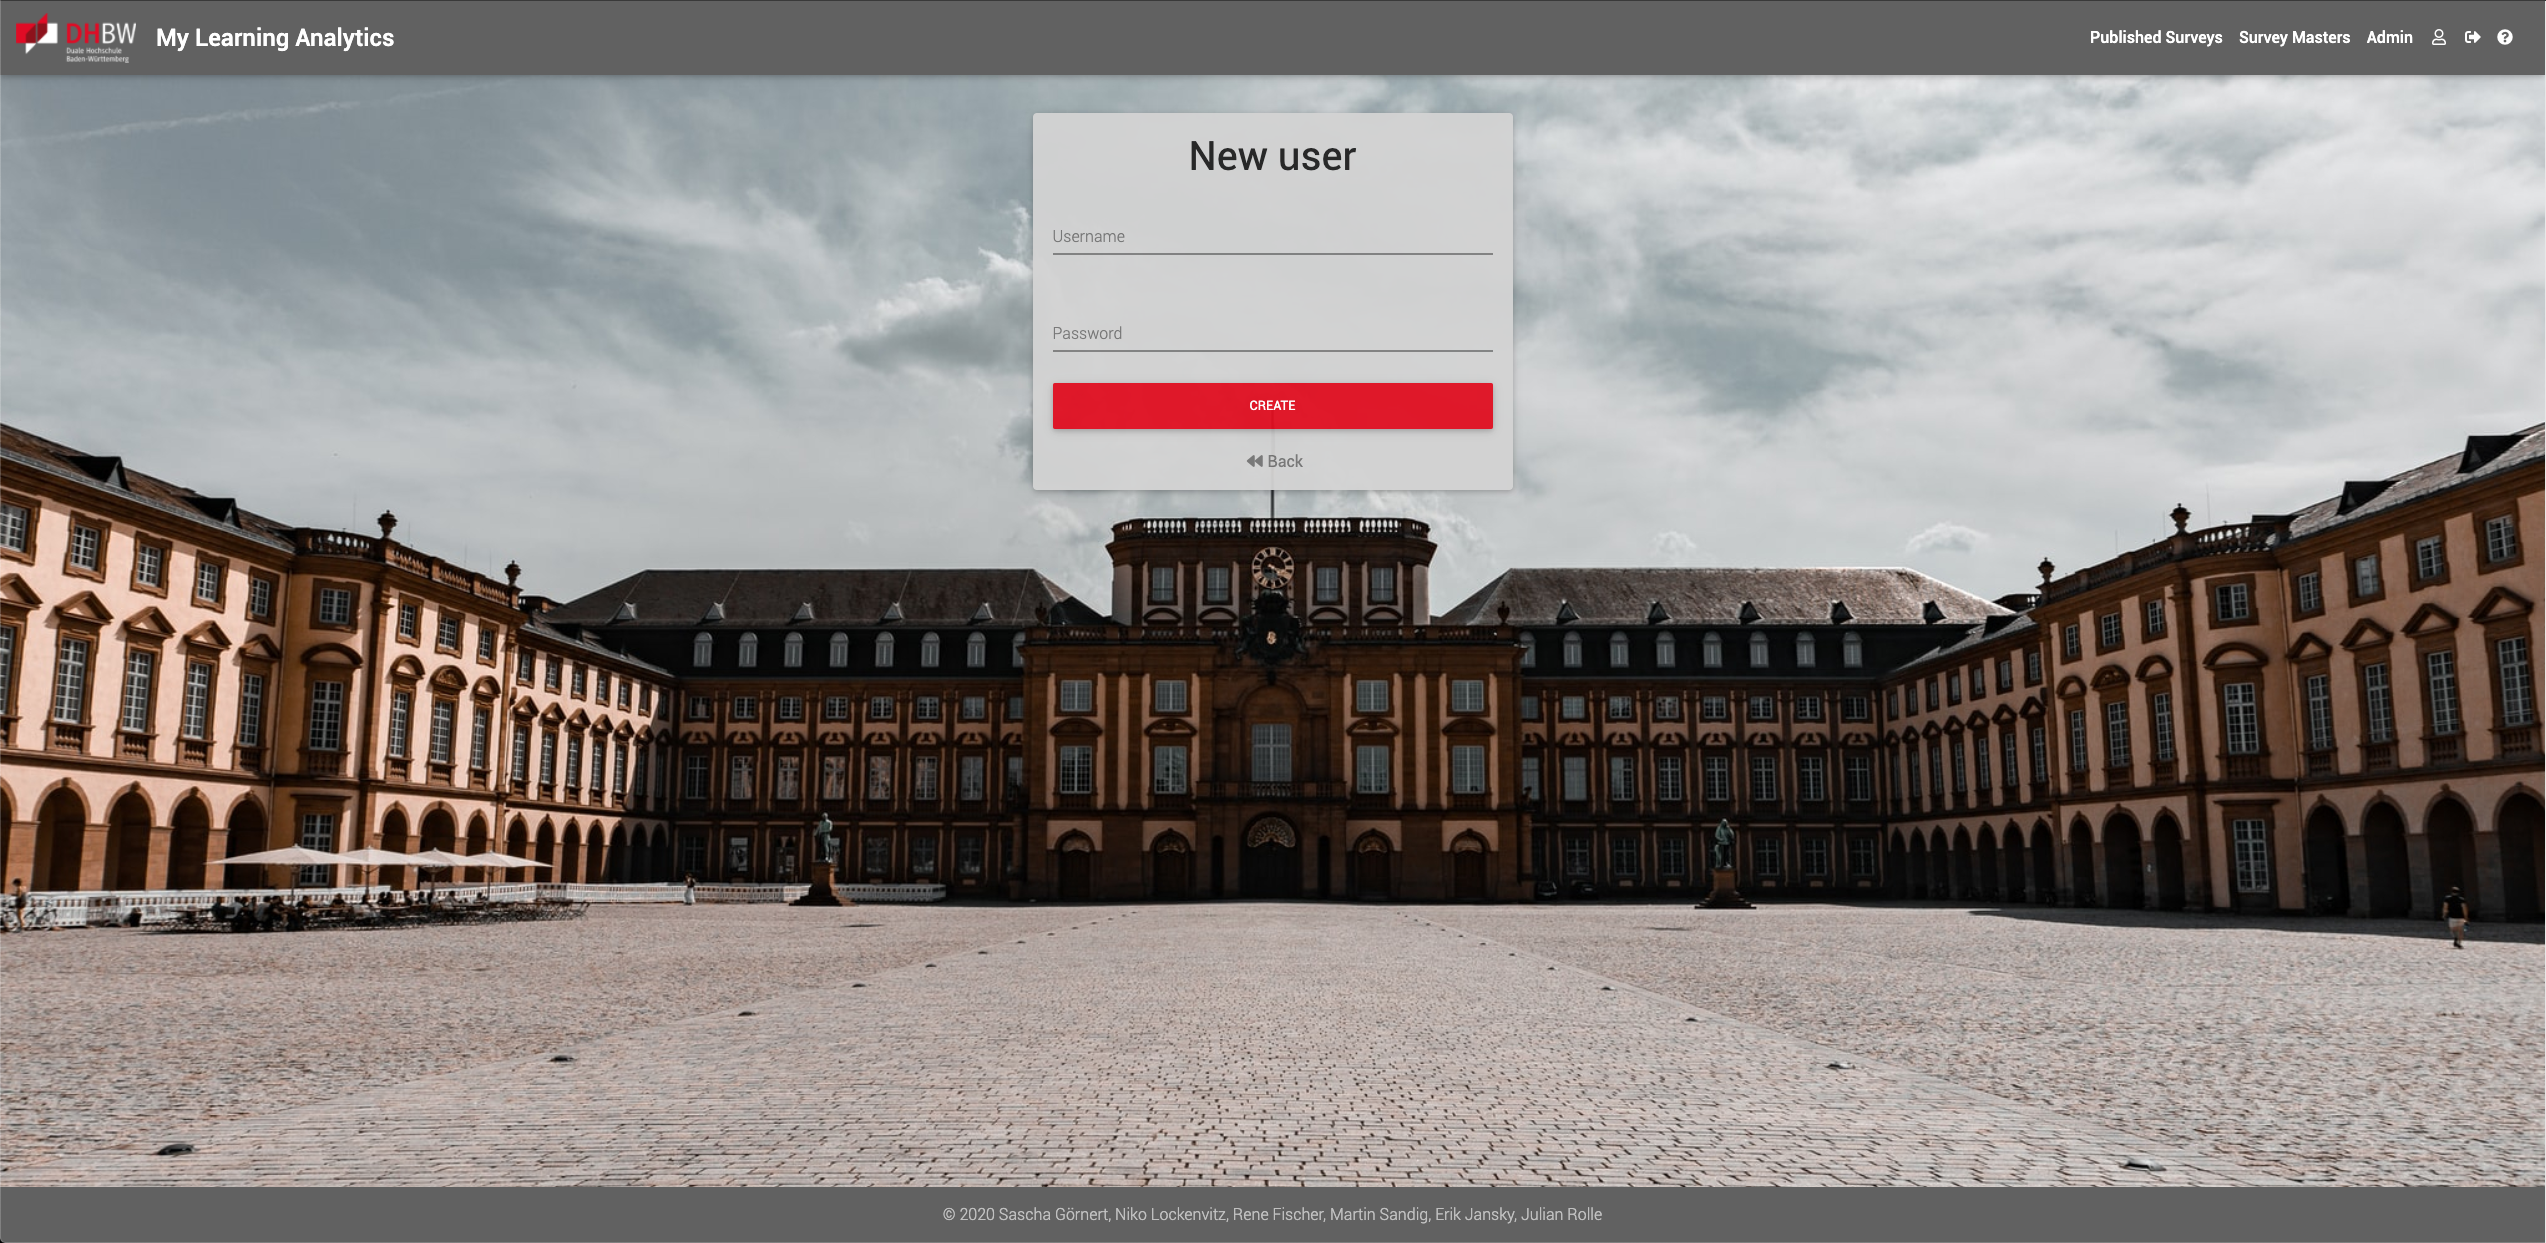
\includegraphics[width=0.95\textwidth, keepaspectratio]{img/client/AdminCreateUser.png}
	\captionsetup{justification=centering, format=plain}
	\caption[\acl{UI}: Neuen Benutzer der Anwendung hinzufügen]{\acl{UI}: Neuen Benutzer der Anwendung hinzufügen \\ \quelleScreenshot}
	\label{fig:AdminCreateUserImplement}
\end{figure}
